\documentclass[xcolor={usenames,svgnames,x11names,table}]{beamer}

\usetheme{SBU}

\usepackage{mypackages}
\usepackage{mycommands}
\colorlet{syn}{SteelBlue4!90!black}
\colorlet{phon}{SeaGreen4}
\colorlet{morph}{Purple}

\forestset{
  visible on/.style={
    for tree={
      /tikz/visible on={#1},
      edge={/tikz/visible on={#1}}}}}

\title[Tutorial]{%
    Computational Phonology Workshop}
\subtitle{Introduction \& Tutorial}
\author[Graf]{Thomas Graf}
\institute{Stony Brook University\\\texttt{mail@thomasgraf.net}\\\texttt{http://thomasgraf.net}}
\date{Dec 12, 2016}


\begin{document}
\unnumbered{
\begin{frame}
	\titlepage
\end{frame}
}

\unnumbered{
\begin{frame}{Outline}
   \tableofcontents
\end{frame}
}

\section[Subregular Phonology]{The Subregular Enterprise}

\begin{frame}{Computational View of Language}
    In formal language theory, string sets are classified according to their formal complexity.
    %
    \begin{center}
        \begin{tikzpicture}
            \node[fill=orange!90] (box) at (0,0)
                {%
                    \(
                        \color{white}
                        \text{regular} < \text{context-free} < \text{mildly context-sensitive} < \cdots
                    \)
                };

            \node (phon) [below=1em of box, font={\bfseries\color{phon}}] {Phonology};
            \node (morph) [below=1em of phon, font={\bfseries\color{morph}}] {Morphology};
            \node (syn) [below=1em of morph, font={\bfseries\color{syn}}] {Syntax};

            \draw<2->[-{Latex[length=.5em]},thick,phon]
                (phon) -|
                node [pos=.75,right,font={\scriptsize}] {\citecolor{\citet{KaplanKay94}}}
                ($(box.south west) + (2.5em,.2em)$);
            \draw<3->[-{Latex[length=.5em]},thick,morph]
                (morph) -|
                node [pos=.65,right,font={\scriptsize}] {\citecolor{\citet{Karttunen.etal92}}}
                ($(box.south west) + (1.5em,.2em)$);
            \draw<4->[-{Latex[length=.5em]},thick,syn]
                (syn) -|
                node [pos=.6,right,font={\scriptsize}] {\citecolor{\citet{Shieber85}}}
                ($(box.south) + (4.5em,.2em)$);
        \end{tikzpicture}
    \end{center}
    %
    \uncover<5>{%
    This allows predictions for
    %
    \begin{itemize}
        \item typology
        \item learning
        \item cognitive architecture
    \end{itemize}
    }
\end{frame}

\begin{frame}{Implications of Formal Complexity}
    \begin{columns}
        \column{.7\linewidth}
        \citet{HeinzIdsardi11, HeinzIdsardi13} highlight\\
        the implications:
        %
        \begin{itemize}
            \item different typology\\
                  \subpoint{center embedding, crossing dependencies}
            \item different memory architecture\\
                  \subpoint{flat \& finite VS unbounded nested stacks}
            \item different learning algorithms\\
                  \subpoint{much harder for syntax}
        \end{itemize}

        \column{.25\linewidth}
        \centering
        \scriptsize
        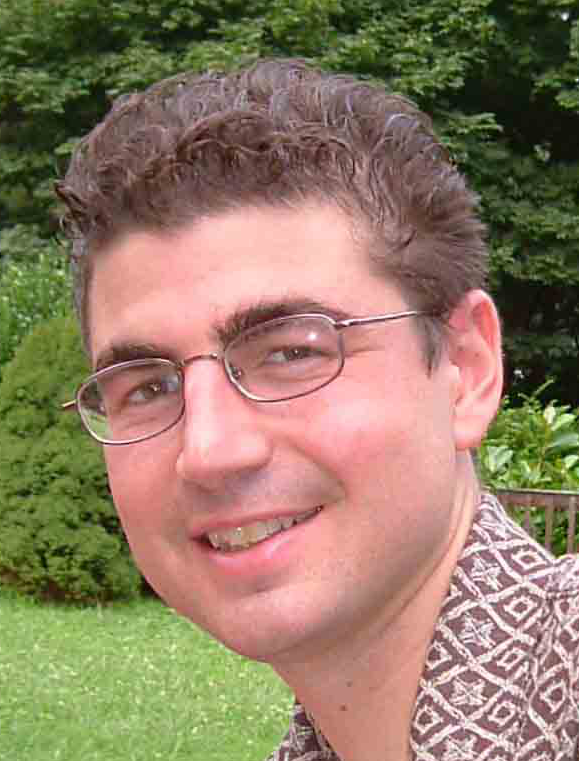
\includegraphics[width=1\linewidth]{./img/heinz_crop}\\

        \bigskip
        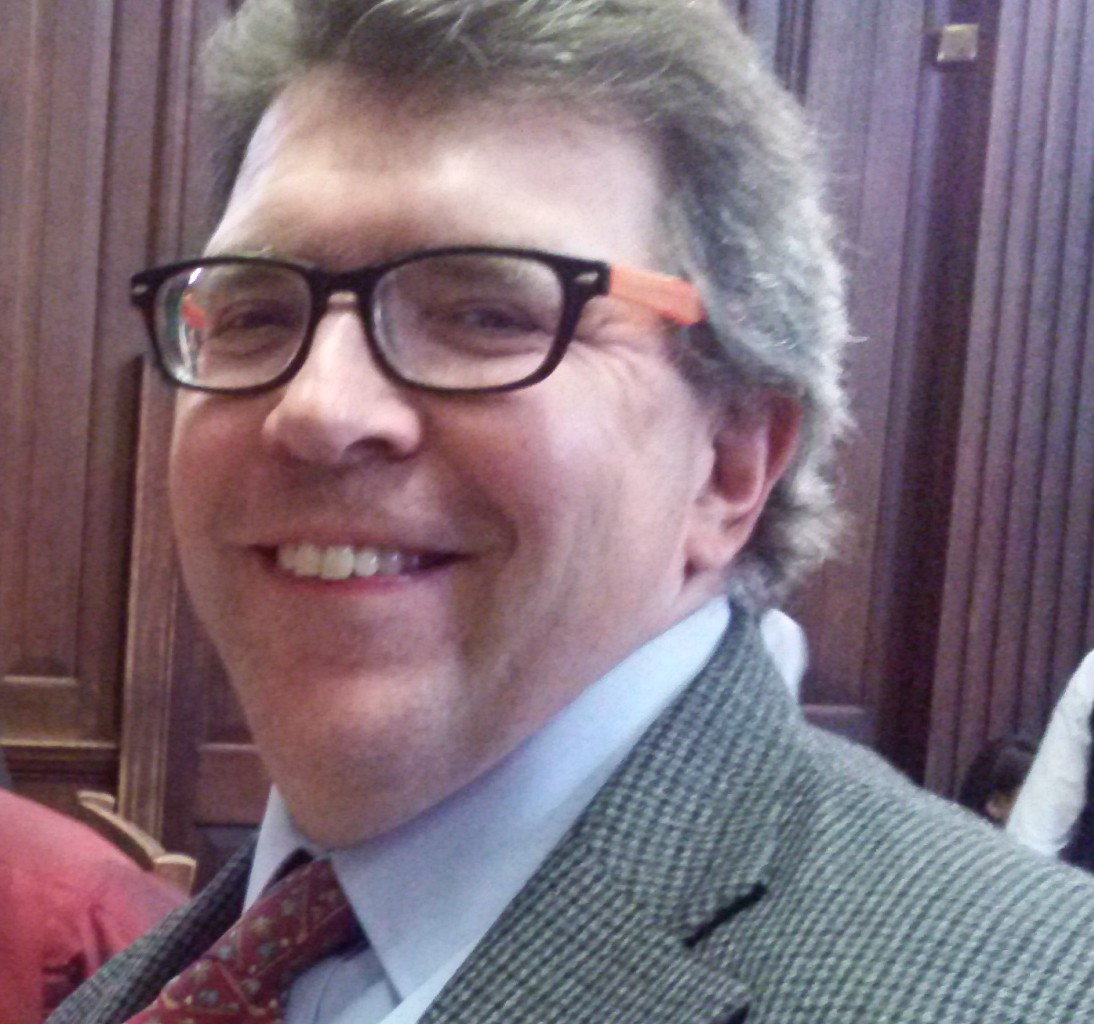
\includegraphics[width=1\linewidth]{./img/idsardi}\\
    \end{columns}
>>>>>>> d5ba3cd716b0cbadc1ad522be937109c5a2c07ae
\end{frame}

\begin{frame}{Too Many Patterns are Regular}
    \begin{itemize}
        \item \textbf{Problem}
            \begin{itemize}
                \item All phonological and morphological patterns are regular.
                \item But not all regular patterns occur in phonology.
            \end{itemize}
        \item Regularity is \highlight{too loose an upper bound}.
    \end{itemize}
    %
    \pause
    \begin{example}
        \begin{itemize}
            \item First-last consonant harmony
            \item Every word with a plosive contains an open syllable
            \item Word with at least 3 suffixes must have exactly 5 prefixes
        \end{itemize}
    \end{example}
\end{frame}

\begin{frame}{Subregular Languages}
    Often forgotten: hierarchy of \highlight{subregular languages}\\
    \citecolor{\citep{McNaughtonPappert71,Rogers.etal10, RuizEtAl98, RogersPullum11, Heinz.etal11, Graf16Phonology}}
    %
    \begin{center}
        \begin{tikzpicture}
            % hierarchy
            \node (REG) at (0,0) {REG};
            \node (SF) [below right=2em of REG] {SF\slash DBSP};
            \node (dummy) [left=5.5em of SF] {\phantom{SL}};
            \node (LTT) [below=1em of dummy] {LTT};
            \node (LT) [below=1em of LTT] {LT};
            \node (SL) [below=3em of LT] {SL};
            \node (SLT) at ($(SL) !.5! (LT)$) [xshift=-3em] {SLT};
            \node (SP) [right=5.5em of SL] {SP};
            \node (PT) [above=3em of SP,xshift=3em] {PT};
            \node (IBSP) [above=2em of SP,xshift=-1.5em] {IBSP};
            \node (TSL) [below=9em of REG,xshift=-1em] {TSL};

            % edges
            \foreach \Source/\Target in {%
                SL/LT,
                SL/TSL,
                SL/SLT,
                SLT/LT,
                SP/PT,
                SP/IBSP,
                PT/SF,
                TSL/IBSP,
                IBSP/SF,
                LT/LTT,
                LTT/SF,
                SF/REG%
            }
            \draw (\Source) to (\Target);

            % highlight
            \node [fit=(SL)(SP)(IBSP),
             draw=orange, fill=orange!75, opacity=.2, thick,
             visible on=<2->] {};
            %
            \node [fit=(SL)(TSL), xshift=.2em, yshift=.2em,
             draw=purple, fill=purple!75, opacity=.2, thick,
             visible on=<3>] {};
        \end{tikzpicture}
    \end{center}
\end{frame}

\section[Phonotactics]{(Tier-Based) Strictly Local Phonotactics}

\begin{frame}{SL: Strictly Local}
    \begin{itemize}
        \item SL formalizes \highlight{local dependencies}.
        \item SL grammars are collections of markedness constraints\\
            that are
            %
            \begin{itemize}
                \item hard\slash non-violable,
                \item locally bounded.
            \end{itemize}
    \end{itemize}

    \begin{block}{Strictly Local Grammars \& Languages}
        \begin{description}
            \item[SL$_n$ grammar] finite set of forbidden $n$-grams
            \item[SL$_n$ language] all strings except those with forbidden $n$-grams
        \end{description}
    \end{block}
\end{frame}

\begin{frame}{Example: SL Constraints}
    \begin{center}
        \begin{tabular}{rll}
            \textbf{Process} & \textbf{Constraint} & \textbf{Forbidden $n$-grams}\\
            Word-final devoicing
            &
            \Constraint{\Purple{[+voice]}\Teal{\RE}}
            &
            \Purple{z}\Teal{\RE},
            \Purple{v}\Teal{\RE}, \ldots
            \\[12pt]
            %
            Intervocalic voicing
            &
            \Constraint{\Teal{V}\Purple{[-voice]}\Teal{V}}
            &
            \Teal{a}\Purple{s}\Teal{a},
            \Teal{a}\Purple{s}\Teal{i},
            \ldots,
            \Teal{i}\Purple{s}\Teal{a},
            \Teal{i}\Purple{s}\Teal{i},
            \ldots,\\
            &
            &
            \Teal{a}\Purple{f}\Teal{a},
            \Teal{a}\Purple{f}\Teal{i},
            \ldots,
            \Teal{i}\Purple{f}\Teal{a},
            \Teal{i}\Purple{f}\Teal{i},
            \ldots,
            \\[12pt]
            %
            CV template
            &
            \Constraint{\Teal{\LE}\Purple{V}}
            &
            \Teal{\LE}\Purple{a},
            \Teal{\LE}\Purple{i},
            \ldots
            \\
            &
            \Constraint{\Teal{C}\Purple{C}}
            &
            \Teal{p}\Purple{p},
            \Teal{p}\Purple{b},
            \ldots
            \Teal{b}\Purple{p},
            \Teal{b}\Purple{b},
            \ldots
            \\
            &
            \Constraint{\Teal{V}\Purple{V}}
            &
            \Teal{a}\Purple{a},
            \Teal{a}\Purple{i},
            \ldots,
            \Teal{i}\Purple{a},
            \Teal{i}\Purple{i},
            \ldots
            \\
            &
            \Constraint{\Purple{C}\Teal{\RE}}
            &
            \Purple{p}\Teal{\RE},
            \Purple{b}\Teal{\RE},
            \ldots
        \end{tabular}
    \end{center}
\end{frame}

\begin{frame}{SL is Too Weak}
    \begin{itemize}
        \item SL grammars only handle unbounded dependencies.
        \item But some processes in phonology are unbounded.
    \end{itemize}
    %
    \begin{exampleblock}{Samala Sibilant Harmony \citep[16]{Heinz15}}
        \begin{tabular}{r@{\hspace{.1em}}l}
                               & \textesh tojonowonowa\textesh\\
            \visible<2->{$^*}$ & \visible<2->{stojonowonowa\textesh}\\
            \visible<2->{$^*}$ & \visible<2->{\textesh tojonowonowas}
        \end{tabular}
    \end{exampleblock}
\end{frame}

\begin{frame}{TSL: Tier-Based Strictly Local}
    We can make Samala SL-like if we \highlight{create new locality domains}.
    %
    \begin{block}{Tier-Based Strictly Local Grammars \& Languages}
        \begin{description}
            \item[TSL$_n$ grammar] finite set of forbidden $n$-grams + tier alphabet
            \item[TSL$_n$ language] all strings except those with forbidden $n$-grams over tier
        \end{description}
    \end{block}

    \begin{center}
        \begin{forest}
            [,phantom,for tree={grow'=90}
                [\textbf{\{b,c\}-Tier:}, l=5.5em]
                [\LE,name=le
                    [\LE,name=tle]
                ]
                [a]
                [b,name=b1
                    [b,name=tb1]
                ]
                [a]
                [c,name=c1
                    [c,name=tc1]
                ]
                [a]
                [a]
                [a]
                [b,name=b2
                    [b,name=tb2]
                ]
                [\RE,name=re
                    [\RE,name=tre]
                ]
                % some white space
                [,phantom]
                % grammar
                [$^*$bcb,l=4em,name=ngram,draw=purple,thick,fill=Purple!75,opacity=.2]
            ]
            %
            \node [fit=(tb1)(tc1)(tb2),draw=Purple,thick,fill=Purple!75,opacity=.2] (illicit) {};
            \draw[Purple!75,thick] (illicit) |- ($(ngram)+(0em,4em)$) -- (ngram);
        \end{forest}
    \end{center}
\end{frame}

\begin{frame}{Example: Sibilant Harmony}
    %fixme: redo examples from Samala
    \begin{center}
        \begin{tabular}{l@{\hspace{2em}}l}
            \textbf{Constraint} & \textbf{Forbidden $n$-grams on sibilant tier}\\
            %
            \Constraint{\Teal{[$\alpha$ ant]} $\cdots$ \Purple{[$-\alpha$ ant]}}
            &
            \Teal{\textipa{\textesh}}\Purple{\textipa{s}},
            \Teal{\textipa{s}}\Purple{\textipa{\textesh}}
        \end{tabular}
    \end{center}

    \bigskip
    \begin{center}
        \begin{tikzpicture}[text height=1em]
    \node (1) at (0,0) {\LE};

    \foreach \Node/\Ref/\Label in {2/1/e,
                                   3/2/\textipa{\textesh},
                                   4/3/i,
                                   5/4/s,
                                   6/5/i,
                                   7/6/\RE}
        \node (\Node) [right=.25em of \Ref] {\Label};

    \node (tier-1) [above=1em of 1] {\LE};
    \node (tier-3) [above=1em of 3] {\Teal{\textipa{\textesh}}};
    \node (tier-5) [above=1em of 5] {\Purple{s}};
    \node (tier-7) [above=1em of 7] {\RE};

    \node (label-base) [left=2em of 1] {\textbf{Base:}};
    \node (label-base) [left=2em of tier-1] {\textbf{Tier:}};

    \foreach \Node in {1,3,5,7}
        \draw (\Node) to (tier-\Node);
\end{tikzpicture}


        \bigskip
        \begin{tikzpicture}[text height=1em]
    \node (1) at (0,0) {\LE};

    \foreach \Node/\Ref/\Label in {2/1/e,
                                   3/2/\textipa{\textesh},
                                   4/3/i,
                                   5/4/\textipa{\textesh},
                                   6/5/i,
                                   7/6/\RE}
        \node (\Node) [right=.25em of \Ref] {\Label};

    \node (tier-1) [above=1em of 1] {\LE};
    \node (tier-3) [above=1em of 3] {\Teal{\textipa{\textesh}}};
    \node (tier-5) [above=1em of 5] {\Teal{\textipa{\textesh}}};
    \node (tier-7) [above=1em of 7] {\RE};

    \node (label-base) [left=2em of 1] {\textbf{Base:}};
    \node (label-base) [left=2em of tier-1] {\textbf{Tier:}};

    \foreach \Node in {1,3,5,7}
        \draw (\Node) to (tier-\Node);
\end{tikzpicture}

    \end{center}
\end{frame}

\begin{frame}{Example: Stress Assignment}
    %fixme: typeset examples in forest
    \begin{description}
        \item[Culminativity] every word has exactly one primary stress
    \end{description}
    
    \bigskip
    \begin{tabular}{rl}
        \textbf{Tier} & contains segments with primary stress\\
        \textbf{$n$-grams}         & \Teal{ś}\Purple{ś} and \Teal{\LE\RE}
    \end{tabular}

    \bigskip
    \begin{center}
        \begin{tikzpicture}
    \node (1) at (0,0) {\LE};

    \foreach \Node/\Ref/\Label in {2/1/a,
                                   3/2/l,
                                   4/3/a,
                                   5/4/\RE}
        \node (\Node) [right=.25em of \Ref] {\Label};

    \node (tier-1) [above=1em of 1] {\LE};
    \node (tier-5) [above=1em of 5] {\RE};

    \foreach \Node in {1,5}
        \draw (\Node) to (tier-\Node);
\end{tikzpicture}

        \hspace{2em}
        \begin{tikzpicture}
    \node (1) at (0,0) {\LE};

    \foreach \Node/\Ref/\Label in {2/1/á,
                                   3/2/l,
                                   4/3/á,
                                   5/4/\RE}
        \node (\Node) [right=.25em of \Ref] {\Label};

    \node (tier-1) [above=1em of 1] {\LE};
    \node (tier-2) [above=1em of 2] {á};
    \node (tier-4) [above=1em of 4] {á};
    \node (tier-5) [above=1em of 5] {\RE};

    \foreach \Node in {1,2,4,5}
        \draw (\Node) to (tier-\Node);
\end{tikzpicture}


        \medskip
        \begin{tikzpicture}
    \node (1) at (0,0) {\LE};

    \foreach \Node/\Ref/\Label in {2/1/á,
                                   3/2/l,
                                   4/3/a,
                                   5/4/\RE}
        \node (\Node) [right=.25em of \Ref] {\Label};

    \node (tier-1) [above=1em of 1] {\LE};
    \node (tier-2) [above=1em of 2] {á};
    \node (tier-5) [above=1em of 5] {\RE};

    \foreach \Node in {1,2,5}
        \draw (\Node) to (tier-\Node);
\end{tikzpicture}

        \hspace{2em}
        \begin{tikzpicture}
    \node (1) at (0,0) {\LE};

    \foreach \Node/\Ref/\Label in {2/1/a,
                                   3/2/l,
                                   4/3/á,
                                   5/4/\RE}
        \node (\Node) [right=.25em of \Ref] {\Label};

    \node (tier-1) [above=1em of 1] {\LE};
    \node (tier-4) [above=1em of 4] {á};
    \node (tier-5) [above=1em of 5] {\RE};

    \foreach \Node in {1,4,5}
        \draw (\Node) to (tier-\Node);
\end{tikzpicture}

    \end{center}
\end{frame}

\begin{frame}{What TSL Cannot do}
    
\end{frame}

\begin{frame}{Attested Patterns Beyond TSL?}
    A few other patterns may go beyond TSL.
    %
    \begin{itemize}
        \item \textbf{Non-Final RHOL} \highlight{[Baek's talk]}\\
        \item \textbf{Multiple Harmony} \highlight{[Aks\"{e}nova's talk]}\\
    \end{itemize}
\end{frame}

\begin{frame}{Complexity of Phonology}
    \begin{itemize}
        \item All local phonological constraints are SL\@.
        \item All segmental long-distance constraints are TSL\@.\\
        \item Suprsegmental constraints (tone, stress) may go beyond TSL\@.\\
            \citecolor{\citep{Graf10PLC, Graf10Thesis, Jardine15}}
    \end{itemize}
\end{frame}

\begin{frame}{Cognitive Implications}
    \begin{itemize}
        \item SL and TSL languages are \highlight{learnable} from positive data.\\
        \citecolor{\citep{Heinz.etal12,JardineHeinz16}}
            \begin{itemize}
                \item UG: specifies upper bound on size of $n$-grams
                \item memorize which sequences have not been seen so far
                \item induce tier (more complex)
                \item learning input can be relatively small
            \end{itemize}
        \item What cognitive resources are required?\\
            \begin{itemize}
                \item Only memorization of the last $n$ segments of a specific type
                \item For most processes $n \leq 3$, and for all $n \leq 7$
                \item Fits \highlight{within bounds of human working memory}
            \end{itemize}

    \end{itemize}
\end{frame}

\begin{frame}{Interim Summary: Phonotactics}
    \begin{itemize}
        \item Natural languages have \highlight{TSL phonotactics}. 
        \item gives tighter bound on typology
        \item solves poverty of stimulus by greatly simplifying learning
        \item reduces cognitive resource requirements
    \end{itemize}

    \pause
    \begin{block}{Next}
        \begin{itemize}
            \item phonological mappings
            \item SL \& TSL syntax
        \end{itemize}
    \end{block}
\end{frame}

\section[Mappings]{Subregular Mappings for Phonology}

\begin{frame}{Phonological Mappings}
    \begin{itemize}
        \item So far we have only considered phonotactics.
        \item But mappings from underlying representations to\\
            surface forms can be studied, too.
        \item Regular mappings are enough.\\
            \citecolor{\citep{KaplanKay94}}
        \item What about subregular mappings?
    \end{itemize}
\end{frame}

\begin{frame}{Input Strictly Local Mappings}
    \begin{block}{Input Strictly Local (ISL)}
        \begin{itemize}
            \item Move through string from left to right.
            \item Rewrite $x$ as $y$ based on previous $n$ symbols in input string.
            \item Output is \highlight{not considered}!
        \end{itemize}
    \end{block}
    %
\end{frame}

\begin{frame}{A Note on TSL}
    Every TSL$_n$ grammar can be decomposed into
    \begin{enumerate}
        \item an \highlight{ISL$_1$} function (the tier projection), and
        \item an SL$_n$ grammar.
    \end{enumerate}

    \pause
    \begin{block}{An Interesting Puzzle}
        \begin{itemize}
            \item What happens if we use an ISL$_k$ function for tier projection?
            \item Addressed in \highlight{Aniello De Santo}'s talk
        \end{itemize}
    \end{block}
\end{frame}

\section[Syntax]{(Tier-Based) Strictly Local Syntax}

\begin{frame}{(Tier-Based) Strictly Local Syntax}
    \begin{itemize}
        \item SL tree grammars are common in computational linguistics:
            \highlight{context-free grammars}
        \item By adding tier projection, we get TSL tree grammars.
    \end{itemize}

    \begin{exampleblock}{Example: CFGs as SL$_2$ Tree Grammars}
        \begin{columns}
            \column{.35\linewidth}
            \begin{tabular}{rcl}
                 S & $\rightarrow$ & NP VP\\
                NP & $\rightarrow$ & John\\
                VP & $\rightarrow$ & cried\\
            \end{tabular}

            \column{.5\linewidth}
            \begin{forest}
                [S [NP] [VP] ]
            \end{forest}
            %
            \begin{forest}
                [NP [John]]
            \end{forest}
            %
            \begin{forest}
                [VP [cried]]
            \end{forest}
        \end{columns}
    \end{exampleblock}
\end{frame}

\begin{frame}{Example: An Illicit Tree}
    \textbf{SL$_2$ Tree Grammar}\\
        \begin{center}
            \small
            \begin{tabular}{cccccc}
                \begin{forest}
                    [S, for tree={parent anchor=south, child anchor=north}
                        [NP]
                        [VP]
                    ]
                \end{forest}
                &
                \begin{forest}
                    [NP, for tree={parent anchor=south, child anchor=north}
                        [N]
                    ]
                \end{forest}
                &
                \begin{forest}
                    [N, for tree={parent anchor=south, child anchor=north}
                        [cats]
                    ]
                \end{forest}
                &
                \begin{forest}
                    [VP, for tree={parent anchor=south, child anchor=north}
                        [V]
                        [NP]
                    ]
                \end{forest}
                &
                \begin{forest}
                    [V, for tree={parent anchor=south, child anchor=north}
                        [bite]
                    ]
                \end{forest}
                &
                \begin{forest}
                    [N, for tree={parent anchor=south, child anchor=north}
                        [dogs]
                    ]
                \end{forest}
            \end{tabular}
        \end{center}

    \begin{columns}
        \column{.4\linewidth}
        \textbf{Example Tree}\\
            \small
            \centering
            \begin{forest}
                [S, for tree={parent anchor=south, child anchor=north}
                    [NP,
                        [N,
                            [dogs]
                        ]
                    ]
                    [VP,
                        [V,
                            [bite]
                        ]
                        [NP,
                            [N,
                                [dogs]
                            ]
                        ]
                        [NP,
                            [N,
                                [dogs]
                            ]
                        ]
                    ]
                ]
            \end{forest}
        \column{.6\linewidth}
        \textbf{Tree Bigrams of Example Tree}\\
            \small
            \quad
            \begin{tabular}{cccc}
                \begin{forest}
                    [S, for tree={parent anchor=south, child anchor=north}
                        [NP]
                        [VP]
                    ]
                \end{forest}
                &
                \begin{forest}
                    [NP, for tree={parent anchor=south, child anchor=north}
                        [N]
                    ]
                \end{forest}
                &
                \begin{forest}
                    [N, for tree={parent anchor=south, child anchor=north}
                        [dogs]
                    ]
                \end{forest}
                &
                \begin{forest}
                    [V, for tree={parent anchor=south, child anchor=north}
                        [bite]
                    ]
                \end{forest}
                \\
                \color{red}
                \begin{forest}
                    [VP, for tree={parent anchor=south, child anchor=north}
                        [V]
                        [NP]
                        [NP]
                    ]
                \end{forest}
            \end{tabular}
    \end{columns}
\end{frame}

\begin{frame}{Tier Projection for Trees}
    Just as for strings, we can project tiers for trees.\\
    \citecolor{\citep{GrafHeinz16JOLLI}}
    %
    \begin{center}
        \begin{forest}
            [,phantom, s=5em,grow'=100
                [S, for tree={parent anchor=south, child anchor=north}
                    [NP,
                        [N,
                            [dogs,name=d1]
                        ]
                    ]
                    [VP,name=vp
                        [V,
                            [bite]
                        ]
                        [NP,
                            [N,
                                [dogs,name=d2]
                            ]
                        ]
                        [NP,
                            [N,
                                [dogs,name=d3]
                            ]
                        ]
                    ]
                ]
                [{\rotatebox[origin=c]{90}{$\ltimes$}},name=t
                    [dogs,name=td1]
                    [VP,name=tvp
                        [dogs,name=td2]
                        [dogs,name=td3]
                    ]
                ]
            ]
            %
            \foreach \Node in {d1,d2,d3}
                \draw[dotted,thick,teal,opacity=.6] (\Node) to (t\Node);
            \draw[dotted,thick,teal,opacity=.6] (vp) to [out=15,in=160] (tvp);
            \node [left=.1em of t,teal] {\textbf{\{dogs,VP\}-Tier:}};
        \end{forest}
    \end{center}
\end{frame}

\begin{frame}{Towards TSL-Syntax}
    While TSL-Syntax is still young, it holds promise:
    \begin{itemize}
        \item movement dependencies are TSL \citecolor{\citep{GrafHeinz16JOLLI}}
        \item Mandarin negation in \highlight{Hongchen Wu's talk}
        \item scope ambiguities in \highlight{Lei Liu's blitz talk}
    \end{itemize}
\end{frame}


\section*{Conclusion}
\subsection*{Conclusion}
\begin{frame}{Conclusion}

\end{frame}

\appendix
\begin{frame}[allowframebreaks]{References}
    \scriptsize
    \def\newblock{}
    \bibliography{./bib/yale2016}
    \bibliographystyle{./bib/linquiry3}
\end{frame}
\end{document}
